\documentclass[conference]{IEEEtran}
\IEEEoverridecommandlockouts

% ---------- Packages ----------
\usepackage{cite}
\usepackage{amsmath,amssymb,amsfonts}
\usepackage{graphicx}
\usepackage{textcomp}
\usepackage{xcolor}
\usepackage{booktabs}
\usepackage{array}
\usepackage{tabularx}
\usepackage{listings}
\usepackage{xurl}
\usepackage[hidelinks]{hyperref}

\def\BibTeX{{\rm B\kern-.05em{\sc i\kern-.025em b}\kern-.08em
    T\kern-.1667em\lower.7ex\hbox{E}\kern-.125em X}}

\newcolumntype{Y}{>{\raggedright\arraybackslash}X}
\renewcommand{\arraystretch}{1.12}

\lstset{
  basicstyle=\ttfamily\scriptsize,
  breaklines=true,
  breakatwhitespace=false,
  columns=fullflexible,
  frame=single,
  xleftmargin=2pt,
  xrightmargin=2pt
}

\begin{document}

\title{Token-Aware Agentic Architecture for Cospas-Sarsat Alert Intelligence:\\
Predictable Cost, Protected Safety}
\author{
    \IEEEauthorblockN{Smruti Rout} \\
    \IEEEauthorblockA{
        \textit{Software Architect \& AI Researcher} \\
        Bengaluru, Karnataka, India \\
        Email: \texttt{smruti.srr@gmail.com} \\
        \vspace{0.2cm}
        \small White Paper --- October 2026 \\
        \textit{Reference Use Case: An Alert Intelligence Agent at 8,000 Assessments per Day}
    }
    \thanks{Independent analysis. This paper is not an official Cospas-Sarsat publication, and the architecture it describes is a proposal, not a programme specification. Every cost figure is reproducible with the accompanying Python script (Appendix A). Dollar figures use 2024-era list prices for the models named; re-run the script with current prices before using them for budgeting.}
}

\maketitle

% =====================================================================
\begin{abstract}
AI agents can support first-line triage of Cospas-Sarsat distress alerts, but an agent re-submits its goal and history at every step, and every tool call adds another full re-read, so token cost grows with every alert handled. This paper proposes a token-aware agentic control plane that combines tiered model routing, prompt caching and context compaction with automatic escalation, outcome-based cost telemetry and a read-only tool gateway. The agent runs beside the alert path, is advisory only, and fails open to a human controller. Using published list prices and a transparent four-step pipeline at 8,000 assessments per day, the modelled cost of a tool-free workflow falls from \$0.1182 to \$0.0376 per assessment, a 68.2\% reduction worth about \$235,000 a year. Letting the correlation step call tools nearly doubles the cost of the cheap design, to \$0.0721 per assessment, yet that is still 72.2\% below a naive premium agent with the same tools (about \$547,000 a year), provided the gateway trims results, caching stays intact and a ceiling bounds the number of tool rounds. The savings survive pessimistic cache and failure assumptions, and compaction overtakes caching on long investigations. Prices are 2024-era and scenario inputs are assumptions to be replaced with pilot data. The paper also sets out safety invariants, governance metrics, a phased roadmap and a reproducible calculation script.
\end{abstract}

\begin{IEEEkeywords}
Cospas-Sarsat, search and rescue, LLM agents, tool use, token economics, prompt caching, model routing, FinOps
\end{IEEEkeywords}

% =====================================================================
\section{Introduction and Summary of Findings}
\label{sec:intro}

An AI agent that triages Cospas-Sarsat alerts can cost 68\% less than a premium-model-only design without touching the safety path: in our modelled deployment, spend falls from \$0.1182 to \$0.0376 per assessment, about \$235,000 a year at 8,000 assessments a day. Letting that agent call tools raises the bill, but the same disciplines keep it 72\% below a naive tool-using agent (Section~\ref{sec:tools-econ}).

The case for triage support is strong. The Cospas-Sarsat System turns 406~MHz beacon activations into alert and location data for rescue authorities, and it has assisted in rescuing about 67,000 people since 1982, to the end of 2024 \cite{paris}. Yet the programme's own statistics show that most alerts reaching SAR services are not genuine emergencies: in 2019 the average SAR false alert rate, which counts false and undetermined alerts together, was 96.65\%, roughly one real alert in 30 \cite{far}. First-line verification is therefore a large share of a rescue coordinator's work, and it must be done while treating every alert as real until proven otherwise.

AI agents are well suited to that evidence-gathering work, but they are expensive in a way chatbots are not. An agent re-submits its goal, scratchpad and prior reasoning at every step. A 2026 Stanford Digital Economy Lab study of agentic coding tasks found that agents consumed about 1,000 times more tokens than code reasoning or chat, and that repeated runs of the same task differed by up to 30 times in total tokens \cite{bai}. Those are coding benchmarks, not alert triage, but the mechanism is the same: the whole context is re-read at every step. Left ungoverned, that cost scales with every alert.

This paper applies a \emph{Token-Aware Control Plane} to the problem: intelligent model routing, prompt caching and context compaction, backed by automatic escalation, outcome-based FinOps telemetry and a read-only tool gateway for the steps where the model chooses its own evidence. Using published API prices and a transparent four-step pipeline, I find:
\begin{itemize}
\item \textbf{68.2\% lower cost} than a premium-by-default design (the tool-free workflow of Sections~\ref{sec:usecase} to~\ref{sec:econ}): \$345,144 falls to \$109,679 per year, a saving of \textbf{\$235,465} for one workflow.
\item \textbf{Routing alone saves 34.6\%.} Prompt caching removes a further \textbf{51.4\%} of what remains, because the SAR procedures prompt is large (6,000 tokens) and identical on every run.
\item \textbf{The failure accounting is conservative.} Failed cheap-model attempts are billed in full, and the premium baseline is given no failure penalty. The resulting escalation tax is 20.4\%. Two other assumptions run the other way (a 100\% cache hit rate and no cache-write fee), which is why Section~\ref{sec:robust} stress-tests them.
\item \textbf{The saving is robust.} It stays at 56.6\% even if the cheap model fails 60\% of the time, and at 51.4\% if the cache serves only half of the static prompt. Routing alone stops paying only when the cheap model fails about 80\% of the time.
\item \textbf{For long investigations, compaction overtakes caching.} On a 40-step case-monitoring agent, caching saves 28\%, compaction 35\%, and the two together 63\%.
\item \textbf{Tools nearly double the cheap design's bill, and the design still pays.} Letting Step 2 call tools through a read-only gateway raises the cost from \$0.0376 to \$0.0721 per assessment (+91.9\%). That is 72.2\% below a naive premium agent with the same tools (\$210,463 against \$757,740 a year) and 39.0\% below the tool-free premium workflow. A tool-call ceiling bounds the worst case at 2.3 times the mean.
\end{itemize}

Cost control must never compete with safety. The architecture keeps the agent \textbf{beside the alert path, never in it}; humans make every decision; no step that judges distress likelihood runs on the cheapest tier; every tool is read-only; and when any budget limit is hit the system \textbf{fails open to a human controller} with the raw alert intact.

The lesson for leaders is that token volume is a cost metric, not a value metric. The measure that matters is cost per assessed alert, set against the controller time and certainty it buys.

% =====================================================================
\section{Context: Why Alert Triage Is a Token Problem}
\label{sec:context}

\subsection{How the Alerting Chain Works}

Cospas-Sarsat is an intergovernmental programme of 45 Participants (May 2025) \cite{wg11}. Beacons such as EPIRBs, ELTs and PLBs transmit at 406~MHz; satellites in low-Earth, geostationary and medium-Earth orbit relay the signals to ground stations; Mission Control Centres (MCCs) distribute the resulting alert data to Rescue Coordination Centres (RCCs) and other SAR points of contact. Cospas-Sarsat provides the data. It does not itself conduct search-and-rescue operations. The Secretariat also maintains the International Beacon Registration Database (IBRD), which lets responders identify who owns a beacon and whom to call. The medium-Earth-orbit (MEOSAR) system reached its initial operational capability in April 2023 \cite{wg10}.

The human impact is concrete. In 2024, Cospas-Sarsat alert data assisted in 1,171 distress incidents and 3,211 persons were rescued \cite{wg11}. These are the rescues; behind them sits a far larger flow of alerts that turn out not to be emergencies.

\subsection{The Triage Burden}
\label{sec:triage}

Cospas-Sarsat measures a SAR false alert rate: false alerts plus undetermined alerts (no person in distress found, or no beacon found) as a share of alerts transmitted to SAR services. The rate was stable from 2015 to 2019, between 96.30\% and 96.85\%, averaging 96.65\% in 2019 \cite{far}, and was 95.55\% in 2020 \cite{sartf2}. Earlier status papers note that ELT beacons contribute disproportionately, and that correct beacon registration greatly improves the chance of resolving an alert quickly. About 3.17 million 406~MHz beacons were deployed in 2023, roughly three-quarters of them GNSS-capable \cite{baku}, so the volume of alert data to reconcile is large and steady.

One principle governs all of this work: \textbf{an alert is treated as real until it is confirmed false.} That principle shapes our architecture. An AI agent may enrich, rank and recommend. It may never close, suppress or delay.

\subsection{Why Agents Break the Chatbot Cost Model}
\label{sec:agents}

A chatbot is one query, one call, one answer. An agent is a loop, and three mechanics change the economics:
\begin{enumerate}
\item \textbf{State carrying.} Each step resubmits the whole history, including the goal, prior reasoning and tool results, so input context grows with every step and cumulative billed tokens grow faster than the step count.
\item \textbf{Input-dominated cost.} In the premium-by-default baseline of Section~\ref{sec:three}, input tokens account for 77.2\% of cost, because the agent keeps re-reading procedures, schemas and registry records to make small decisions. The Stanford study reports the same pattern in coding agents \cite{bai}.
\item \textbf{Stochastic volatility.} Depending on whether the agent finds an efficient path or gets stuck in a reasoning loop, the same job can vary by up to 30 times in total tokens \cite{bai}. Budgeting on averages alone is unsafe.
\end{enumerate}

\subsection{Three Traps}

\begin{itemize}
\item \textbf{The leaderboard misconception.} Ranking people or teams by tokens consumed rewards burning tokens, not resolving cases.
\item \textbf{Premium by default.} Wiring every step to the strongest model is simple, and at scale most steps (parsing, formatting) never needed it.
\item \textbf{Savings that touch safety.} The most dangerous optimisation is the one that quietly lowers the quality of a life-safety judgement. Section~\ref{sec:invariants} sets out invariants that cost control may not cross.
\end{itemize}

% =====================================================================
\section{The Use Case: An Alert Intelligence Agent}
\label{sec:usecase}

\subsection{Scenario}

A regional hub (an MCC and its supported RCCs) deploys an agent that performs first-line assessment each time a new alert arrives or a material update changes an existing one. It returns a structured case brief that a human controller reviews: who the beacon is registered to, whether it has a history of false activations, how it correlates with other detections and context, how likely the alert is to be genuine, and which verification actions to take first. The alert itself is forwarded to the RCC at once, exactly as it is today; the brief follows alongside it. The pipeline has four steps (Table~\ref{tab:steps}).

\begin{table*}[!t]
\caption{The Four-Step Assessment Pipeline}
\label{tab:steps}
\centering
\footnotesize
\begin{tabularx}{\textwidth}{@{}l l Y Y l@{}}
\toprule
\textbf{Step} & \textbf{Task} & \textbf{Detail} & \textbf{Complexity} & \textbf{Tier} \\
\midrule
1 & Parse & Decode and normalise the alert message; classify beacon type and activation context & Low (extraction, classification) & Tier 1 (lite) \\
2 & Correlate and assess & Assess the prefetched registry record and history; call read-only tools for further evidence (other detections, vessel or aircraft track, weather, drift) as the findings require; estimate likelihood of genuine distress; recommend checks & High (multi-source reasoning, ambiguity, tool use) & Tier 2 (core) \\
3 & Structure & Build the schema-valid case payload for the RCC case-management system & Low to medium, schema-sensitive & Tier 1 (lite) \\
4 & Verify & Consistency and safety validation before a controller sees the brief; confirm nothing was suppressed & High (safety-critical) & Tier 2 (core) \\
\bottomrule
\end{tabularx}
\end{table*}

\emph{Design note on Step 1.} Where alert messages arrive in a fixed, specified format, parse them with deterministic code and pass the result to the model as data. Reserve the Tier 1 model for normalisation and classification, so that a misread position or beacon identifier cannot originate in a language model.

\emph{Workflow versus agent.} Steps 1, 3 and 4 run in a fixed order, so the pipeline is a routed workflow: the router chooses the tier and the controller decides on retries, but the model never chooses what happens next. Step 2 is where autonomy lives. It is a bounded observe-and-act loop in which the Tier 2 model decides which read-only tool to call next, reads the result, and decides whether it has enough evidence to write the assessment, all inside an allowlist, a per-run tool-call ceiling and the safety invariants of Section~\ref{sec:invariants}. Evidence that every assessment needs (the registry record and the beacon's history) is prefetched by deterministic code and included in the 900-token goal. Tools are for follow-ups whose need depends on what was found. The figures in Sections~\ref{sec:econ} and~\ref{sec:long} price this prefetched workflow, which is the cost floor; Section~\ref{sec:tools-econ} prices Step 2 with tool calls enabled.

\subsection{Why This Use Case Is Representative}

It has every feature that makes agent spend hard to control: a heavy static prompt (SAR procedures, output schemas, false-alert playbooks), a mix of easy and hard steps, a strict output schema where cheap models sometimes fail, and high, steady, around-the-clock volume.

\subsection{Modelling Assumptions}
\label{sec:assumptions}

The scenario inputs are illustrative assumptions, not measured Cospas-Sarsat figures. They are stated so that any operator can replace them with pilot data.
\begin{itemize}
\item Static prompt of 6,000 tokens (procedures, schemas, playbooks) and a dynamic goal of 900 tokens (decoded alert, registry record, history).
\item Output per step of 300, 700, 500 and 300 tokens; each step's output is carried into the next step's input.
\item Volume of 8,000 assessments per day, 365 days a year (2.92 million runs).
\item First-attempt failure probability of 15\% on each Tier 1 step and 5\% on each Tier 2 step. A failed Tier 1 step is re-run on the premium model with 40\% more output.
\item \textbf{Failed attempts are billed.} The wasted first attempt is charged in full, which is more conservative than a simple simulator that does not charge for failed attempts (Section~\ref{sec:convention}).
\item Premium-by-default baseline: all four steps on the premium model, no caching, and no failure penalty.
\item Prompt caching applies to the static prefix only, with a 100\% hit rate in the base case (Section~\ref{sec:robust} varies it).
\item Expected costs are computed exactly by enumerating all 16 failure outcomes, then cross-checked with a 200,000-run Monte Carlo simulation.
\end{itemize}

% =====================================================================
\section{Reference Architecture: The Token-Aware Control Plane}
\label{sec:arch}

The control plane sits between the alert-intelligence agent and its model providers and data sources, and makes every model call and tool call cheaper, more reliable and more observable without changing the agent's business logic. It runs beside the alert-forwarding path, never on it. Fig.~\ref{fig:arch} shows the two paths: the safety-critical alert path at the top, which is unchanged and human-decided, and the advisory assessment path below it, which receives only a copy of each alert and fails open. Tool calls from Tiers 2 and 3 pass through the tool gateway (component 6) to read-only data sources; Tier 1 has no tool access.

\begin{figure*}[!t]
\centering
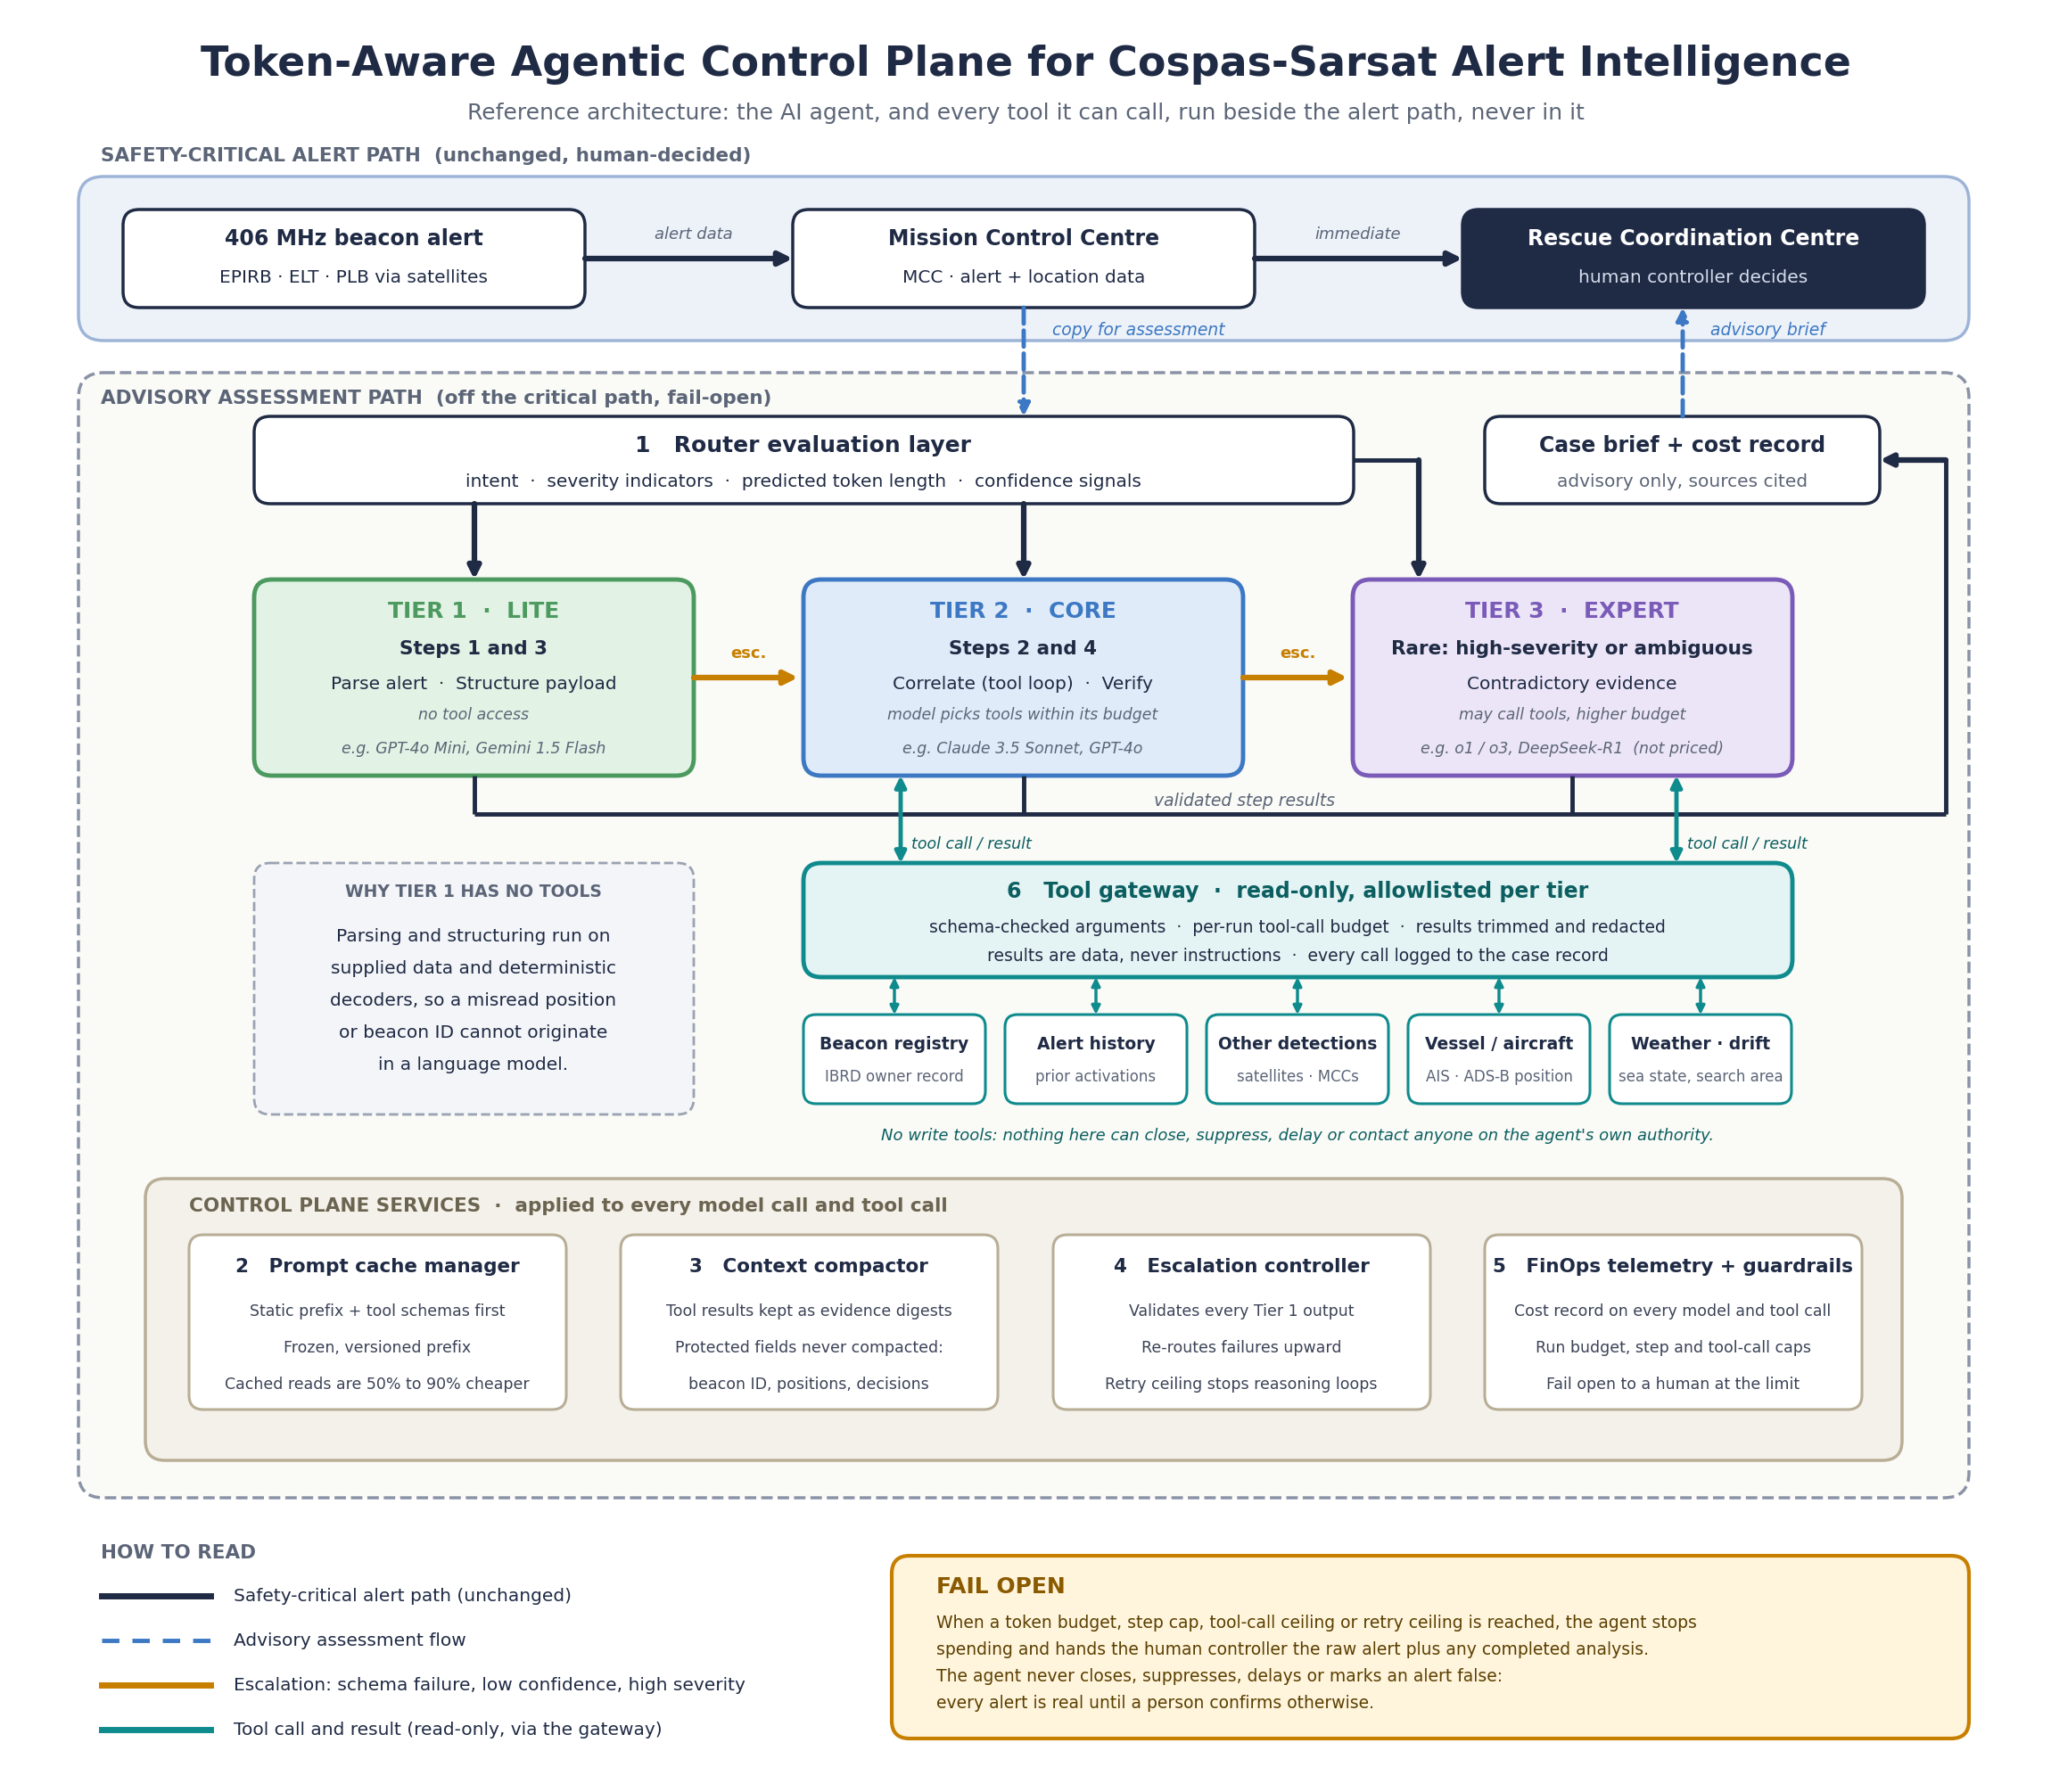
\includegraphics[width=0.88\textwidth]{SAR_Control_Plane_Architecture.png}
\caption{The token-aware control plane. The agent runs beside the alert path, never in it. Numbers 1 to 6 match the components described in Sections~\ref{sec:router} to~\ref{sec:tools}. Tier 1 has no tool access; Tiers 2 and 3 reach read-only data sources only through the gateway.}
\label{fig:arch}
\end{figure*}

\subsection{Component 1: Router Evaluation Layer}
\label{sec:router}

The router sends each step to the cheapest model that can handle it safely. It uses three inputs: intent classification (extraction versus assessment), predicted input length, and confidence and schema-validation signals that trigger escalation. A fourth input is specific to this domain: \textbf{severity indicators} such as an encoded position, a registered vessel or aircraft in a hazardous setting, or corroborating detections. These raise the floor tier and lift budget limits, including the tool-call ceiling (Section~\ref{sec:invariants}).

\begin{table*}[!t]
\caption{Model Tiers and Indicative Cost Profiles}
\label{tab:tiers}
\centering
\footnotesize
\begin{tabularx}{\textwidth}{@{}l Y Y Y@{}}
\toprule
\textbf{Tier} & \textbf{Sample models} & \textbf{Intended work in this use case} & \textbf{Cost profile (per 1M tokens, list price)} \\
\midrule
Tier 1: Lite & GPT-4o Mini, Gemini 1.5 Flash & Alert parsing and normalisation, case-payload structuring & \$0.15 to \$0.35 input; \$0.60 to \$1.50 output \\
Tier 2: Core & Claude 3.5 Sonnet, GPT-4o & Correlation, likelihood assessment, safety verification & \$2.50 to \$3.00 input; \$10.00 to \$15.00 output \\
Tier 3: Expert & OpenAI o1/o3, DeepSeek-R1 & Rare, high-severity or contradictory cases & Variable, with a high compute premium \\
\bottomrule
\end{tabularx}
\end{table*}

Table~\ref{tab:tiers} lists the tiers. Tier 3 is deliberately left out of the cost figures in Section~\ref{sec:econ} because the published pricing gives no fixed price for it. Its use is expected to be rare, and it should be reported as a separate line when measured.

\subsection{Component 2: Prompt Cache Manager}

The SAR procedures, output schemas and false-alert playbooks (6,000 tokens in our scenario) are identical on every call. Prompt caching stores that prefix so the agent pays a fraction of the input price each time it is re-read. The listed discounts are 50\% on cached inputs for OpenAI models and 90\% for Claude 3.5 Sonnet. The manager enforces one discipline: \textbf{static content first, dynamic content last}, with the static prefix versioned and frozen between controlled releases so that the cache stays valid. The tool definitions (about 1,200 tokens in our scenario) are static too, so they join the frozen prefix and are cached with it.

\subsection{Component 3: Context Compactor}

Because state carrying makes input grow with every step, the compactor periodically summarises older history before the next call. It operates only on a defined compactable region. \textbf{Protected fields} (beacon identifier, position and time of each detection, prior assessments and controller decisions) are never summarised away. Tool results are the fastest-growing part of the context, so once a result has been used the compactor replaces it with an evidence digest that keeps its source, timestamp and protected fields. Section~\ref{sec:long} shows why compaction matters for long-running investigations.

\subsection{Component 4: Escalation and Fallback Controller}
\label{sec:escal}

Cheap models are cheap because they are less capable, and they will sometimes fail. The controller validates every Tier 1 output against its schema and assertions. On failure it halts the step, logs the event, and re-routes the exact context payload to a premium model. Tier 2 steps that return low confidence, contradictory evidence or a high-severity indicator escalate to Tier 3 in the same way. A retry ceiling prevents reasoning loops. Every escalation is a recorded signal that the step may be mis-scoped.

\subsection{Component 5: FinOps Telemetry and Guardrails}
\label{sec:finops}

Every model call emits a cost record: model, uncached input, cached input, output, step, run and outcome. Every tool call emits a matching record: tool, result size, latency and outcome. Guardrails use these records to enforce per-run token budgets, step caps, tool-call ceilings and alerts. They are the defence against the 30-times volatility problem, because the worst-case run is bounded and visible rather than discovered on the monthly invoice.


\subsection{Component 6: Tool Gateway}
\label{sec:tools}

An agent differs from a workflow in one respect: the model chooses actions. In this architecture the only actions are read-only lookups, and the model never reaches a data source directly. Every call passes through the tool gateway, which sits between Tiers 2 and 3 and the data sources (Fig.~\ref{fig:arch}). Tier 1 has no tool access: parsing and structuring run on supplied data and deterministic decoders, so a misread position or beacon identifier cannot originate in a language model. Table~\ref{tab:tools} shows an illustrative tool set. Evidence that every assessment needs is prefetched by code from the decoded beacon identifier; the model calls tools only for follow-ups whose need depends on what it has found.

\begin{table*}[!t]
\caption{Illustrative Read-Only Tool Set}
\label{tab:tools}
\centering
\footnotesize
\begin{tabularx}{\textwidth}{@{}l Y Y@{}}
\toprule
\textbf{Tool} & \textbf{Returns} & \textbf{How it is invoked} \\
\midrule
Beacon registry lookup & Registered owner, vessel or aircraft record, contact details (redacted before any external model call) & Prefetched by code from the decoded beacon identifier \\
Alert and activation history & Prior alerts from the same beacon and how each was resolved & Prefetched by code \\
Other detections & Other satellite or MCC detections of the same beacon in the time window & On demand, Tiers 2 and 3 \\
Vessel or aircraft track & Position reports near the detected location (for example AIS or ADS-B) & On demand, Tiers 2 and 3 \\
Weather and sea state & Conditions at the detected position and time & On demand, Tiers 2 and 3 \\
Drift and search-area estimate & A read-only computation from position, time and conditions & On demand, when severity indicators are present \\
\bottomrule
\end{tabularx}
\par\smallskip\footnotesize The list illustrates the pattern. Which sources exist depends on each hub's data agreements, and the table does not describe what any MCC operates.
\end{table*}

The gateway does six jobs:
\begin{enumerate}
\item \textbf{Least privilege.} Read-only credentials and an allowlist per tier and per step. No tool can write, close, suppress, send a message or contact anyone.
\item \textbf{Checked arguments.} Arguments are validated against a schema, and personal data is redacted before any call leaves the hub's approved region.
\item \textbf{Normalised results.} The gateway returns only the fields the step needs, at a bounded size, with a source and a timestamp. In the model of Section~\ref{sec:tools-econ} this trims a raw 1,500-token result to 500 tokens.
\item \textbf{Results are data.} Tool output is delimited and passed as data, never as instructions. Text in a result that looks like an instruction is ignored and logged.
\item \textbf{Budget and timeouts.} A per-run tool-call ceiling (eight rounds in our model, higher for severe alerts) and per-call timeouts, enforced by the controller and not by the model. Reaching the ceiling fails open (invariant~4).
\item \textbf{Evidence ledger.} Every call and result is logged to the case record, and a compact digest goes forward to later steps, so the verifier and the controller can trace each statement in the brief to its source.
\end{enumerate}

\textbf{Who decides what.} The router decides which tier runs a step. The Tier 2 model decides which allowed tool to call next and when it has enough evidence. The controller decides when the budget is spent. A human decides everything that matters for the alert. Only the second of these is autonomy, and it is confined to choosing among read-only lookups.

\subsection{Safety Invariants That Cost Control May Not Cross}
\label{sec:invariants}

These eight rules take precedence over every optimisation in this paper.
\begin{enumerate}
\item \textbf{Off the critical path.} The agent never gates, delays or replaces alert forwarding. If the agent is slow, wrong or down, controllers still receive every alert exactly as they do today.
\item \textbf{Advisory only.} The agent enriches, ranks and recommends. A human controller makes every decision, and no alert is closed, suppressed or marked false by the agent.
\item \textbf{Severity floor.} Steps that judge likelihood of distress (assessment and verification) never run on Tier 1. Alerts with severity indicators are routed to at least Tier 2, and ambiguous ones to Tier 3. Higher-severity alerts also receive a higher per-run token budget and tool-call ceiling, so cost limits never starve the cases that matter most.
\item \textbf{Fail open.} When a token budget, step cap, tool-call ceiling or retry ceiling is reached, the system stops spending and hands the human controller the raw alert plus whatever analysis is complete. It never aborts silently or drops the case.
\item \textbf{Asymmetric error cost.} A genuine distress ranked as low priority is the failure that matters most. Validation tracks this recall separately, and a release is blocked if any genuine alert in the validation set falls below the controller-review threshold (Section~\ref{sec:govern} explains how to size that set).
\item \textbf{Degraded mode is normal operations.} The control room must be able to work with the agent switched off, and the model layer must support failover across providers.
\item \textbf{Read-only, least-privilege tools.} The agent has no write, send, close or contact capability. Tools are allowlisted per tier and step, arguments are schema-checked and redacted, and tool output is treated as untrusted data, never as instructions.
\item \textbf{Evidence or silence.} Every factual statement in a brief cites a tool result or a supplied record. A tool that fails, times out or returns nothing is reported to the controller as missing evidence; the agent never fills the gap from model memory.
\end{enumerate}

% =====================================================================
\section{The Economics}
\label{sec:econ}

\subsection{Price Points Used}
\label{sec:prices}

Prices are per 1 million tokens, taken from each provider's published pricing \cite{openai,anthropic,google}. They are list prices of earlier model generations, so treat the dollar figures as a worked example of the method. Verify them against current provider documentation before budgeting, as listed prices and model generations change often.

\begin{table*}[!t]
\caption{List Prices Used in the Model (USD per 1M Tokens)}
\label{tab:prices}
\centering
\footnotesize
\begin{tabularx}{\textwidth}{@{}l r r r Y@{}}
\toprule
\textbf{Model} & \textbf{Input} & \textbf{Output} & \textbf{Cached input} & \textbf{Notes} \\
\midrule
OpenAI GPT-4o & \$2.50 & \$10.00 & \$1.25 & 50\% discount on cached inputs \\
Claude 3.5 Sonnet & \$3.00 & \$15.00 & \$0.30 & 90\% savings via prompt caching \\
Gemini 1.5 Pro & \$1.25 & \$5.00 & n/a & Context caching lowers base rates; higher rates apply to very long prompts \\
GPT-4o Mini & \$0.15 & \$0.60 & \$0.075 & Cost-effective for agent micro-steps \\
Gemini 1.5 Flash & \$0.35 & \$1.50 & n/a & Built for speed and ultra-low cost \\
\bottomrule
\end{tabularx}
\end{table*}

The model uses GPT-4o Mini for Tier 1 and Claude 3.5 Sonnet for Tier 2. Sonnet's input costs 20 times Mini's and its output 25 times, and that gap is the economic basis of routing.

\subsection{Three Architectures Compared}
\label{sec:three}

\begin{table*}[!t]
\caption{Cost of the Three Architectures (Exact Expectation over All Failure Outcomes)}
\label{tab:arch}
\centering
\footnotesize
\begin{tabularx}{\textwidth}{@{}l Y r r r r@{}}
\toprule
\textbf{Architecture} & \textbf{Description} & \textbf{Per run} & \textbf{Per 1,000 runs} & \textbf{Per day} & \textbf{Per year} \\
\midrule
A. Premium by default & All four steps on Claude 3.5 Sonnet, no caching & \$0.1182 & \$118.20 & \$946 & \$345,144 \\
B. Routed & Tier 1 / Tier 2 split with escalation, no caching & \$0.0773 & \$77.34 & \$619 & \$225,836 \\
C. Routed and cached & B plus caching of the static prefix & \$0.0376 & \$37.56 & \$300 & \$109,679 \\
\bottomrule
\end{tabularx}
\end{table*}

Architecture A is a deterministic baseline with no failure penalty. B and C pay for every escalation, including the wasted first attempt. The comparison is therefore tilted against the proposed design on failure accounting, and the savings are conservative in that respect (Table~\ref{tab:arch}). These three architectures price the tool-free workflow, with the registry record and history prefetched into the goal; Section~\ref{sec:tools-econ} adds tool calls.

Fig.~\ref{fig:cost} shows where each architecture's money goes. Input tokens are 77.2\% of the baseline bill, which is why routing and caching, both of which attack input cost, are so effective. In architecture C the wasted first attempts cost only about \$1.75 per 1,000 assessments.

\begin{figure}[!t]
\centering
\includegraphics[width=\columnwidth]{chart2_cost_composition.png}
\caption{Cost per 1,000 assessments by architecture, split into full-price input, cached input, output and billed first attempts that failed. Modelled outcome at 8,000 assessments a day (Section~\ref{sec:assumptions}).}
\label{fig:cost}
\end{figure}

\subsection{Where the Savings Come From}
\label{sec:savings}

\begin{itemize}
\item \textbf{Routing alone: 34.6\% reduction} (\$0.1182 to \$0.0773). Half the steps run on a model about 20 times cheaper on input.
\item \textbf{Caching on top of routing: a further 51.4\% reduction} (\$0.0773 to \$0.0376). The 6,000-token static prompt is re-read on all four steps, and in architecture C a cached read serves 78.8\% of all input tokens (26,400 of 33,521 per run).
\item \textbf{Combined: 68.2\% reduction}, or \textbf{\$235,465 a year} for one workflow. Against a baseline that is also charged the 5\% premium-model failure rate, the combined saving is 69.9\%.
\item \textbf{The escalation tax.} A pipeline whose cheap steps never failed would cost \$0.0312 per run (a 73.6\% reduction). Real escalations raise that by 20.4\%, with about 0.40 escalation or retry events per run. The business gets valid outputs in exchange.
\end{itemize}

Fig.~\ref{fig:bridge} shows the annual bridge from the premium baseline to the routed and cached design. Each lever contributes roughly half of the \$235,465 saving. The saving also scales linearly with volume: doubling the alert-assessment rate doubles the dollar saving without changing the architecture.

\begin{figure}[!t]
\centering
\includegraphics[width=\columnwidth]{chart1_savings_bridge.png}
\caption{Annual model spend for one workflow (2.92 million assessments a year): \$345K falls to \$110K, with routing saving \$119K and caching a further \$116K. Modelled outcome (Section~\ref{sec:assumptions}).}
\label{fig:bridge}
\end{figure}

\subsection{Robustness: Do the Savings Survive Worse Assumptions?}
\label{sec:robust}

The two assumptions most likely to be wrong in a real deployment are the cache hit rate and the Tier 1 failure rate. Both were varied with all else held fixed (Tables~\ref{tab:cache} and~\ref{tab:fail}).

\begin{table}[!t]
\caption{Sensitivity to the Share of the Static Prefix Served from Cache}
\label{tab:cache}
\centering
\footnotesize
\begin{tabular}{@{}l r r@{}}
\toprule
\textbf{Share from cache} & \textbf{Cost per run} & \textbf{Saving vs A} \\
\midrule
100\% & \$0.0376 & 68.2\% \\
90\% & \$0.0415 & 64.9\% \\
75\% & \$0.0475 & 59.8\% \\
50\% & \$0.0575 & 51.4\% \\
0\% (routing alone) & \$0.0773 & 34.6\% \\
\bottomrule
\end{tabular}
\end{table}

\begin{table}[!t]
\caption{Sensitivity to the Tier 1 First-Attempt Failure Rate}
\label{tab:fail}
\centering
\footnotesize
\begin{tabular}{@{}l r r@{}}
\toprule
\textbf{Tier 1 failure rate} & \textbf{Cost per run} & \textbf{Saving vs A} \\
\midrule
5\% & \$0.0345 & 70.8\% \\
15\% (base case) & \$0.0376 & 68.2\% \\
30\% & \$0.0421 & 64.4\% \\
45\% & \$0.0467 & 60.5\% \\
60\% & \$0.0513 & 56.6\% \\
\bottomrule
\end{tabular}
\end{table}

Fig.~\ref{fig:robust} plots both sweeps. The saving falls steadily as either assumption worsens, but it does not collapse.

\begin{figure*}[!t]
\centering
\includegraphics[width=0.72\textwidth]{chart4_robustness.png}
\caption{Saving versus premium by default as the cache share (left) and the Tier 1 failure rate (right) vary. Dark bars mark the base case. Modelled outcome (Section~\ref{sec:robust}).}
\label{fig:robust}
\end{figure*}

Two points of interpretation. First, the figure 51.4\% appears twice for unrelated reasons: caching removes 51.4\% of the routed cost (Section~\ref{sec:savings}), and a 50\% cache hit rate leaves a 51.4\% saving against the premium baseline. Second, because escalation re-runs the same payload on the premium model, a higher failure rate mainly raises cost rather than changing what the controller receives; shadow testing should confirm this. Routing alone (without caching) only becomes more expensive than premium-by-default when Tier 1 fails about \textbf{79.9\%} of the time: at a 100\% failure rate the routed pipeline costs \$0.1309 per run against \$0.1182.

\subsection{Tail Risk}
\label{sec:tail}

Averaging hides danger. The exact 99th-percentile run in architecture C costs \$0.0683, which is 1.82 times the mean, and the worst possible combination of failures costs \$0.1010. The larger risk is a pathological run: if an agent hits the 30-times volatility described in Section~\ref{sec:agents}, a baseline run costs about \$3.55 and the same event in architecture C costs about \$1.13. A per-run ceiling (for example five times the mean, about \$0.19) converts that unbounded exposure into a bounded one. Under invariant~4, hitting the ceiling hands the case to a human; it never discards it.

\subsection{Counting Convention}
\label{sec:convention}

A simpler convention does not charge for a failed first attempt. Following that convention, architecture C would cost \$0.0358 per run, 4.7\% less than the \$0.0376 reported here. This paper uses the higher figure.

% =====================================================================
\section{The Economics of the Tool Layer}
\label{sec:tools-econ}

\subsection{Why Tools Change the Arithmetic}

Each tool call is paid for twice. The model emits a request and the gateway returns a result, and then the next model turn must re-read the whole context, including that result, before it can act. A step with $k$ tool rounds therefore makes $k+1$ model calls, and the result of round $j$ is re-read on each of the $k-j+1$ calls that follow it. Input grows with the square of the number of rounds. This is the state-carrying mechanism of Section~\ref{sec:agents}, now driven by the agent's own choices instead of a fixed pipeline.

\subsection{Added Assumptions}

All assumptions of Section~\ref{sec:assumptions} still apply. The tool layer adds the following, which are as illustrative as the rest.
\begin{itemize}
\item Tool definitions of 1,200 tokens join the Step 2 prefix. They are static, so caching covers them.
\item Step 2 makes three sequential tool rounds in the base case, one call per round, on the Tier 2 model. Each call request costs 100 output tokens.
\item The gateway returns 500 tokens per result. Without the gateway the same result is 1,500 tokens.
\item With the gateway, Steps 3 and 4 receive a 100-token evidence digest per call. A naive agent carries the full transcript forward.
\item If the final assessment fails validation, the wasted call is billed and the call is re-run with 40\% more output, as in Section~\ref{sec:assumptions}.
\item The per-run ceiling is eight tool rounds.
\item Not modelled: fees charged by data providers, tool latency and tool failures (Appendix~\ref{app:notes}).
\end{itemize}

\subsection{Cost of the Agentic Design}

Table~\ref{tab:agentic} compares the tool-using designs with the two workflows of Section~\ref{sec:three}. The naive premium agent (A1) runs every step on the premium model, receives raw tool results, carries the whole transcript forward and uses no caching. Design C1 is the proposal: routing, caching and the gateway.

\begin{table*}[!t]
\caption{Cost of the Tool-Using Designs at Three Tool Rounds (Exact Expectation)}
\label{tab:agentic}
\centering
\footnotesize
\begin{tabularx}{\textwidth}{@{}l Y r r r@{}}
\toprule
\textbf{Design} & \textbf{Description} & \textbf{Per run} & \textbf{Per 1,000 runs} & \textbf{Per year} \\
\midrule
Workflow A & Premium by default, no tools (Table~\ref{tab:arch}) & \$0.1182 & \$118.20 & \$345,144 \\
Workflow C & Routed and cached, no tools (Table~\ref{tab:arch}) & \$0.0376 & \$37.56 & \$109,679 \\
\midrule
A1. Naive premium agent & All steps premium, raw results, full transcript carried, no caching & \$0.2595 & \$259.50 & \$757,740 \\
\ \ A1 with gateway only & A1 plus trimmed results and evidence digests & \$0.2145 & \$214.50 & \$626,340 \\
B1. Routed, gateway & Tier 1 / Tier 2 split plus gateway, no caching & \$0.1736 & \$173.58 & \$506,848 \\
\ \ C1 without gateway & Routed and cached, raw results, full transcript carried & \$0.1074 & \$107.40 & \$313,612 \\
\textbf{C1. Routed, cached, gateway} & \textbf{The proposed design} & \textbf{\$0.0721} & \textbf{\$72.08} & \textbf{\$210,463} \\
\bottomrule
\end{tabularx}
\end{table*}

The proposed design costs 72.2\% less than the naive premium agent: \$210,463 against \$757,740 a year, a saving of \$547,277. Applied in order, the gateway removes 17.3\%, routing a further 19.1\% of the remainder, and caching a further 58.5\% of what is left. The order matters and the shares are not additive. Caching carries most of the saving here, because tool results enlarge the context and the 7,200-token prefix is re-read on every turn: a cached read serves 76.5\% of design C1's input tokens (49,260 of 64,385 per run).

\textbf{The tool tax.} Against the tool-free workflow C, tools add \$34.51 per 1,000 assessments, a rise of 91.9\%, or about \$100,800 a year. That is the price of letting the model decide what evidence to fetch, and Section~\ref{sec:govern} says how to judge whether it is worth paying. Design C1 is still 39.0\% cheaper than the tool-free premium workflow A, so the cheapest tool-using design costs less than the simplest design before routing and caching. With zero tool rounds the model collapses to workflow C within 0.8\% (\$0.0379 against \$0.0376), which is the cost of carrying the tool definitions.

\subsection{Cost Grows Faster than the Number of Rounds}

Fig.~\ref{fig:tools} and Table~\ref{tab:rounds} vary the number of tool rounds in Step 2. In design C1 each extra round costs about \$0.0018 more than the one before it: the first round adds \$0.0096 and the tenth \$0.0258. Total cost is therefore quadratic in rounds. Design C1 stays below the tool-free premium workflow A (\$0.1182) up to five rounds and crosses it at six (\$0.1224).

\begin{table}[!t]
\caption{Cost per Run (USD) by Number of Tool Rounds}
\label{tab:rounds}
\centering
\footnotesize
\begin{tabular}{@{}r r r r@{}}
\toprule
\textbf{Rounds} & \textbf{Naive premium} & \textbf{C1, no gateway} & \textbf{C1 (proposed)} \\
\midrule
0 & 0.1218 & 0.0379 & 0.0379 \\
1 & 0.1629 & 0.0563 & 0.0475 \\
3 & 0.2595 & 0.1074 & 0.0721 \\
5 & 0.3753 & 0.1777 & 0.1038 \\
8 & 0.5850 & 0.3192 & 0.1650 \\
10 & 0.7488 & 0.4375 & 0.2147 \\
\bottomrule
\end{tabular}
\end{table}

\begin{figure*}[!t]
\centering
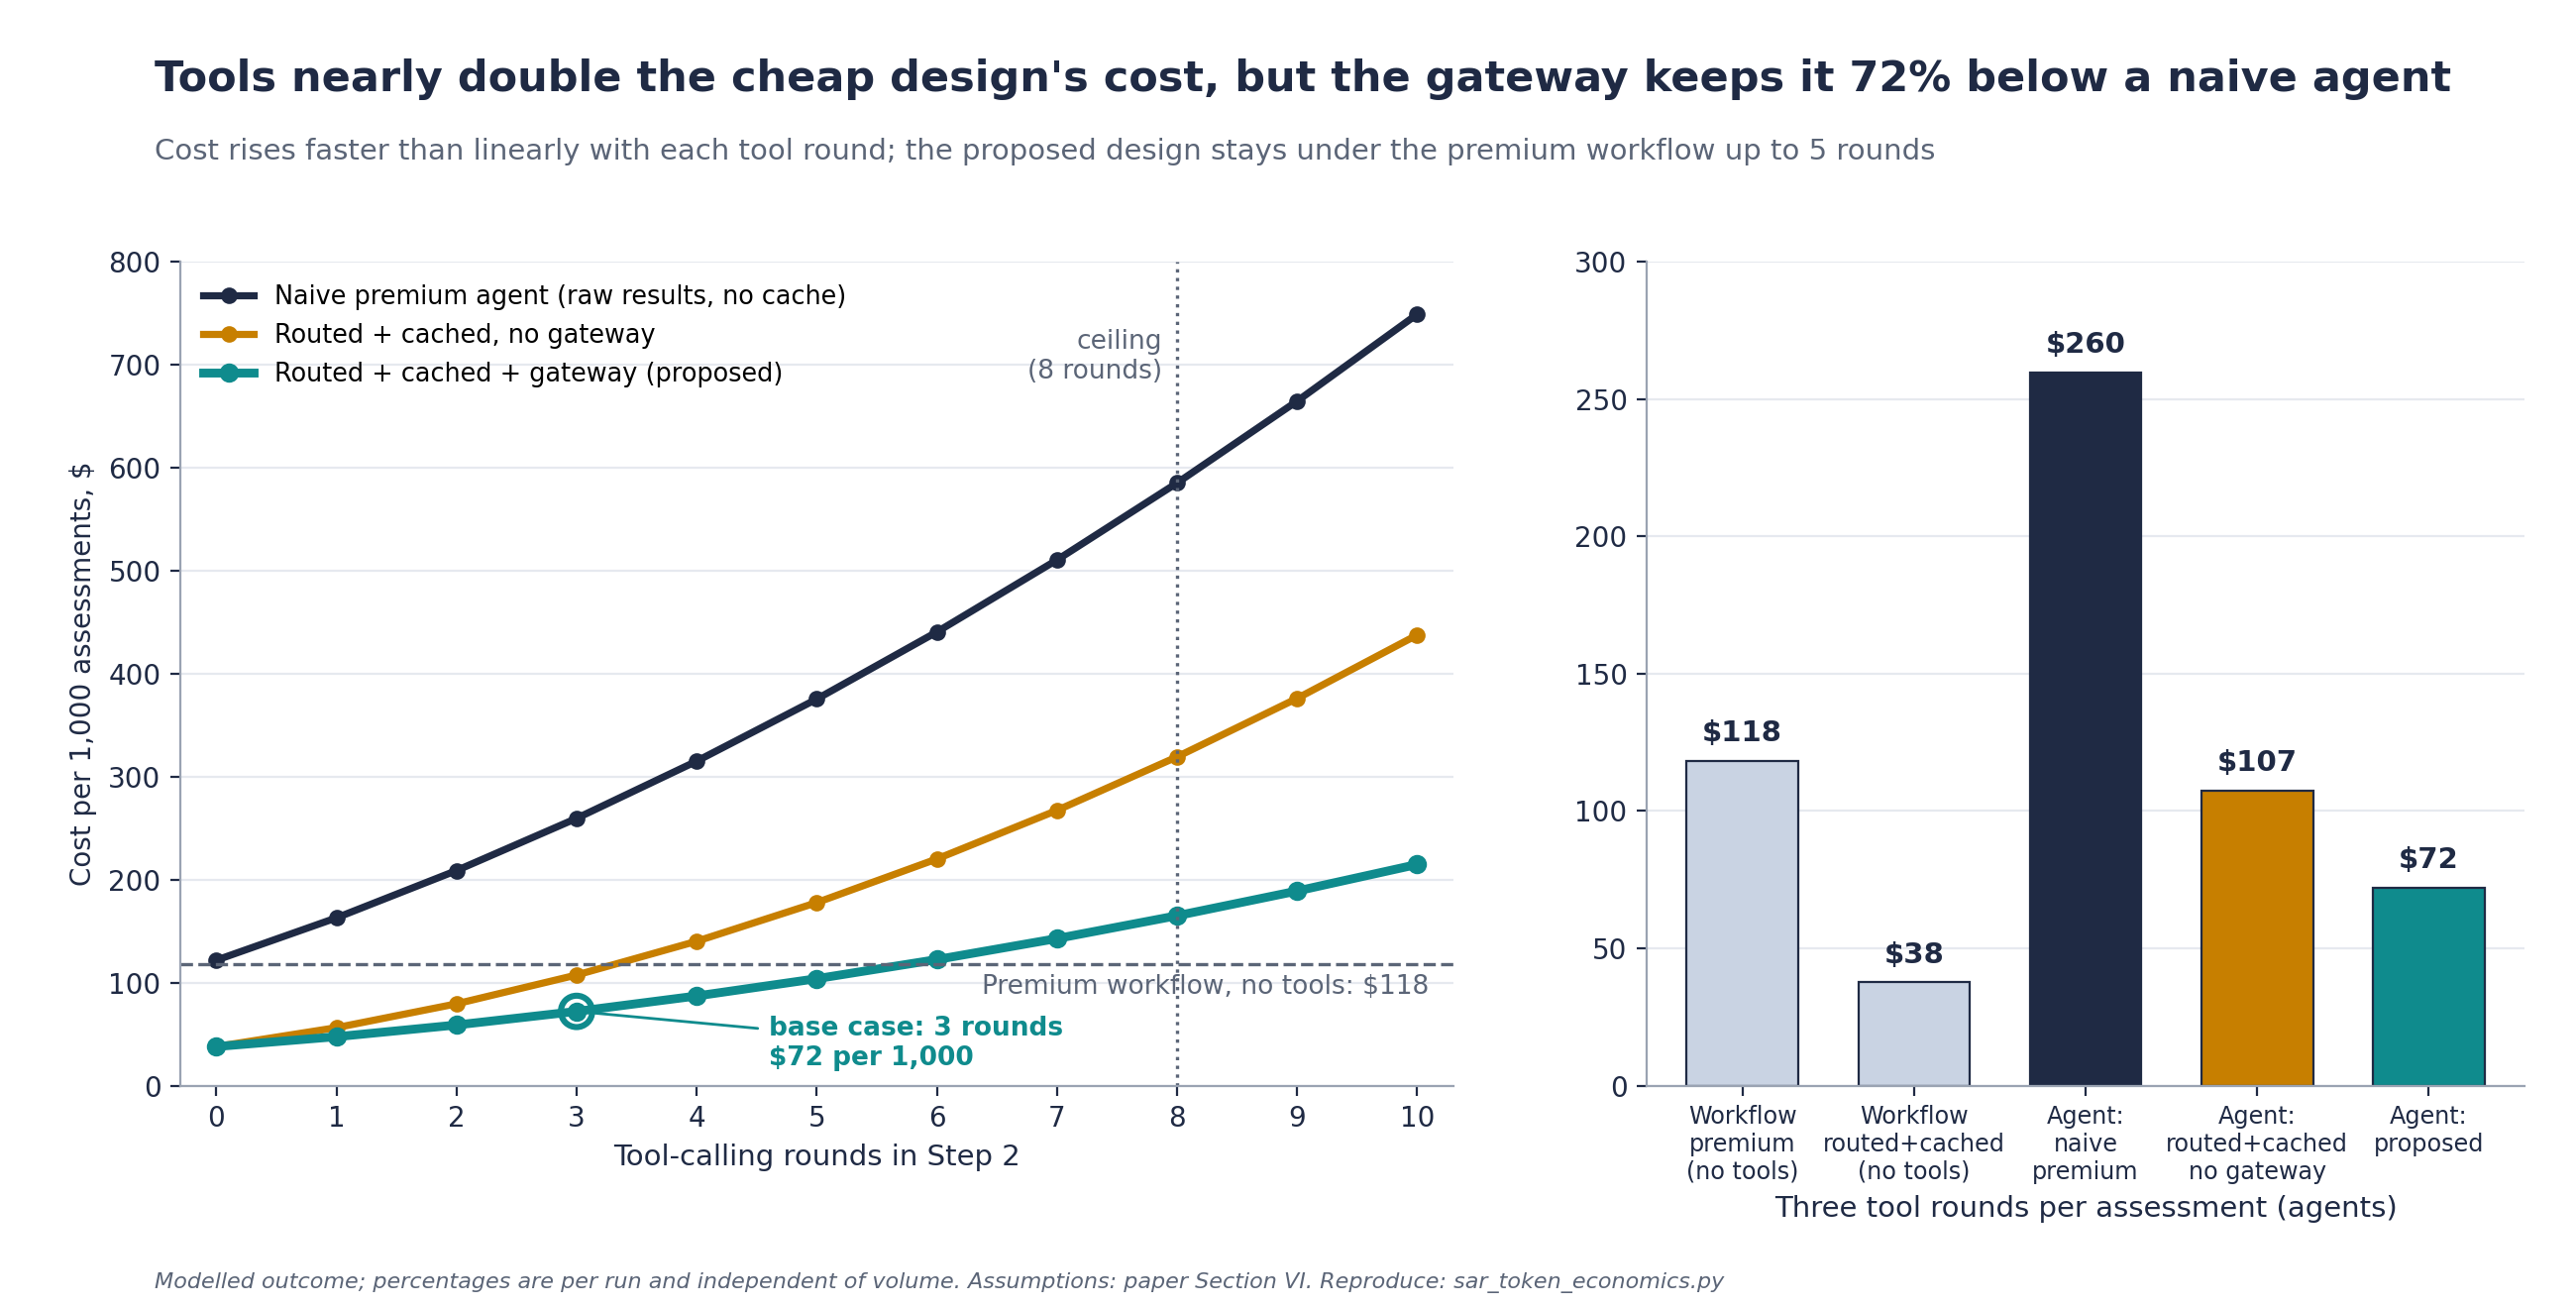
\includegraphics[width=0.86\textwidth]{chart5_tool_layer.png}
\caption{Left: cost per 1,000 assessments as the number of tool rounds in Step 2 grows, for a naive premium agent, a routed and cached agent without the gateway, and the proposed design. Right: the five designs at three rounds. Modelled outcome (Section~\ref{sec:tools-econ}).}
\label{fig:tools}
\end{figure*}

\subsection{Levers Inside the Tool Layer}

\begin{itemize}
\item \textbf{Trim results.} The gateway's trimmed results and digests cut design C1's cost by 32.9\% against raw results (\$0.1074 to \$0.0721). Result size acts directly on cost: each extra 500 tokens per result adds about \$0.0092 per assessment in the base case, and results of 3,000 tokens would raise C1 to about \$0.1182, the cost of the tool-free premium workflow.
\item \textbf{Call in parallel.} Independent lookups (other detections, vessel track, weather) can go in one round. Three calls in one round cost \$0.0550 per assessment, 23.6\% less than three sequential rounds, and also shorten the time to brief.
\item \textbf{Prefetch what is always needed.} Evidence every assessment requires is fetched by code before the model runs, so it costs no model turns.
\item \textbf{Protect the cache.} With tools, a weaker cache hurts far more than in the workflow. At 75\%, 50\% and 0\% of the static prefix served from cache, design C1 costs \$0.0975, \$0.1228 and \$0.1736 per assessment, which is 52.7\% below A1 at 50\% and 33.1\% below it with no caching at all. In the workflow the same 50\% cache share cost \$0.0575.
\end{itemize}

\subsection{Tail Risk with Tools}

The ceiling matters more once the model chooses its own actions. The exact 99th-percentile run in design C1 costs \$0.1089, 1.51 times the mean, and the worst combination of failures costs \$0.1435. A run that uses all eight permitted rounds costs \$0.1650, or 2.29 times the mean. Without a ceiling, an agent that loops for 30 rounds (an illustrative runaway, not a measured one) costs \$1.11 with the gateway and \$2.68 as a naive agent, which is 37.1 times the C1 mean. The ceiling turns that exposure into a bounded one. Under invariant~4, reaching it hands the case to a human with the evidence gathered so far.

\subsection{What the Numbers Do Not Show}

The model prices tool use; it does not value it. Whether the extra evidence improves a controller's decision is an empirical question for the pilot (Section~\ref{sec:govern}). Sequential rounds also add latency to the time to brief, roughly one model round trip plus the tool's own response time per round, which parallel calls and prefetching reduce. Provider fees and tool failures are not modelled. Treat three rounds as a planning assumption, not a measurement. Section~\ref{sec:roadmap} brings tools in only after routing has been measured, so that the number of rounds actually used can replace it.

% =====================================================================
\section{Long-Running Investigations: Why Compaction Matters}
\label{sec:long}

The four-step triage run is short. Some SAR support tasks are not: an agent that follows an evolving case, re-assessing as new detections arrive and drafting situation updates, may run for dozens of steps. The tables below model a premium-model agent with a 6,900-token base context (6,000 static plus 900 goal), 500 tokens of output carried forward at each step, and compaction every 10 steps that replaces history with a 1,000-token summary.

\begin{table}[!t]
\caption{Cumulative Input Tokens with and without Compaction}
\label{tab:tokens}
\centering
\footnotesize
\begin{tabular}{@{}r r r r@{}}
\toprule
\textbf{Steps} & \textbf{Plain} & \textbf{With compaction} & \textbf{Reduction} \\
\midrule
4 & 30,600 & 30,600 & 0\% \\
10 & 91,500 & 91,500 & 0\% \\
20 & 233,000 & 193,000 & 17\% \\
40 & 666,000 & 396,000 & 41\% \\
\bottomrule
\end{tabular}
\end{table}

Ten times as many steps (4 to 40) produce 21.8 times as many input tokens. Because each step re-reads everything before it, input grows roughly with the square of the step count, so cost grows faster than linearly with agent autonomy.

\begin{table}[!t]
\caption{Cost per Run (USD) by Run Length and Optimisation}
\label{tab:longcost}
\centering
\footnotesize
\begin{tabular}{@{}r r r r r@{}}
\toprule
\textbf{Steps} & \textbf{Plain} & \textbf{Caching} & \textbf{Compaction} & \textbf{Both} \\
\midrule
4 & 0.122 & 0.057 & 0.122 & 0.057 \\
10 & 0.350 & 0.188 & 0.350 & 0.188 \\
20 & 0.849 & 0.525 & 0.729 & 0.405 \\
40 & 2.298 & 1.650 & 1.488 & 0.840 \\
\bottomrule
\end{tabular}
\end{table}

Caching saves 53\%, 46\%, 38\% and 28\% across these four run lengths. Compaction saves 0\%, 0\%, 14\% and 35\%. Together they save 53\%, 46\%, 52\% and 63\% (Fig.~\ref{fig:long}).

\begin{figure}[!t]
\centering
\includegraphics[width=\columnwidth]{chart3_caching_vs_compaction.png}
\caption{Cost saving versus a plain premium-model agent at 4, 10, 20 and 40 steps, for caching only, compaction only, and both. Modelled outcome (Section~\ref{sec:long}).}
\label{fig:long}
\end{figure}

\textbf{Architectural insight:} the static prefix is a large share of input in short runs, so caching leads there. As history accumulates, the cached portion shrinks relative to the total and compaction overtakes it; in this scenario the crossover falls between 20 and 40 steps. The two levers are complementary. Short, high-volume triage is caching-led, and long case-following agents need both.

% =====================================================================
\section{Governing for Value, Not Volume}
\label{sec:govern}

Tokens measure cost, not outcomes. The cost side here is small: \$37.56 per 1,000 assessments for the tool-free workflow, and \$72.08 with tools enabled. The value case therefore rests on controller time saved and uncertainty reduced, and those benefits must be measured in a pilot rather than assumed. I recommend replacing token leaderboards with the measures in Table~\ref{tab:metrics}.

\begin{table*}[!t]
\caption{Recommended Governance Metrics}
\label{tab:metrics}
\centering
\footnotesize
\begin{tabularx}{\textwidth}{@{}l Y Y@{}}
\toprule
\textbf{Metric} & \textbf{Definition} & \textbf{Why it matters} \\
\midrule
Genuine-alert recall & Share of genuine alerts in the validation set that the agent ranks above the controller-review threshold & A release gate: the target is no misses \\
Cost per assessed alert & Total model spend divided by assessments delivered & The headline unit economics (\$0.0376 in the base case) \\
Controller agreement and override rate & How often controllers accept the agent's likelihood ranking and recommended checks & Shows whether the agent is actually useful, and whether trust is calibrated \\
Time to brief (p95) & Latency from alert receipt to case brief & Slow briefs are worthless in an emergency; measure it per tier \\
Escalation rate & Share of Tier 1 steps re-routed upward & Early warning that a Tier 1 step is mis-scoped \\
Cache hit ratio & Cached input tokens as a share of all input tokens & Confirms prompt discipline (78.8\% in the base case, which assumes a 100\% hit rate on the static prefix) \\
Tail-run ratio & 99th-percentile run cost divided by the mean & Quantifies volatility exposure (1.82 in the base case) \\
Tool rounds per assessment & Mean and 99th-percentile number of tool-calling rounds in Step 2 & The main driver of agentic cost: the third round adds \$0.0132 in the base case, and every later round costs more \\
Grounding rate & Share of statements in the brief that cite a tool result or a supplied record & Enforces invariant~8; a falling rate means the agent is filling gaps from memory \\
Tool failure rate & Share of tool calls that time out, error or return nothing & Missing evidence degrades the brief and wastes rounds \\
\bottomrule
\end{tabularx}
\end{table*}

\textbf{Sizing the recall gate.} A target of no misses is only meaningful if the validation set is large enough to test it. If a set containing $n$ genuine alerts shows zero misses, the 95\% upper confidence bound on the true miss rate is roughly $3/n$ (the rule of three). Genuine alerts are about one in 30, so a set of 300 genuine alerts, which bounds the miss rate near 1\%, needs roughly 9,000 historical alerts. Plan the validation set, and the length of the shadow phase, around that arithmetic.

Before moving any step to a smaller model, test whether it reaches the same operational outcome at lower cost. A saving that degrades a distress judgement is not a saving. And never reward consumption: reward resolved, well-assessed alerts at lower unit cost.

% =====================================================================
\section{Implementation Roadmap}
\label{sec:roadmap}

Table~\ref{tab:roadmap} gives a phased plan. Caching and instrumentation come first because they carry the least quality risk. Routing is introduced only once measurement is in place, and tools come after routing, because every tool round multiplies the cost of any weakness upstream (Section~\ref{sec:tools-econ}).

\begin{table*}[!t]
\caption{Phased Implementation Roadmap}
\label{tab:roadmap}
\centering
\footnotesize
\begin{tabularx}{\textwidth}{@{}l l Y Y@{}}
\toprule
\textbf{Phase} & \textbf{Timeline} & \textbf{Activities} & \textbf{Exit criterion} \\
\midrule
0. Safety case & Weeks 1 to 3 & Agree the eight invariants with MCC and RCC operators; data-protection and legal review; define the recall target and validation set & Signed safety case and approved data-handling plan \\
1. Instrument and shadow & Weeks 3 to 6 & Run the agent in shadow mode with no operator exposure; log per-call tokens and cost; compare its rankings with actual outcomes & Full cost visibility and a measured baseline cost per assessed alert \\
2. Cache & Weeks 6 to 8 & Restructure prompts as static prefix plus dynamic suffix; enable provider caching; track hit ratio & Cache hit ratio at target with no change in output quality \\
3. Route & Weeks 8 to 12 & Classify steps by complexity; move Tier 1 steps to lite models; add schema validation and escalation; shadow-test against the premium baseline & Genuine-alert recall unchanged; accuracy at tier within tolerance \\
4. Add read-only tools & Weeks 12 to 16 & Build the gateway; start with prefetched lookups only; enable on-demand tools one at a time in shadow mode; measure rounds per assessment, grounding rate and tool failures; set the tool-call ceiling from measured use & Grounding rate at target; cost per assessed alert measured at the real number of rounds; recall unchanged \\
5. Operator pilot & Weeks 16 to 22 & Show briefs to controllers at one RCC; measure time to brief, agreement and override rates & Controllers confirm usefulness; no safety regressions \\
6. Compact, cap and scale & Ongoing & Add compaction for long investigations; set budget ceilings with fail-open behaviour; publish dashboards; extend to further RCCs & Control plane adopted as a shared platform \\
\bottomrule
\end{tabularx}
\end{table*}

% =====================================================================
\section{Risks and Mitigations}
\label{sec:risks}

Table~\ref{tab:risks} lists the principal risks of deploying the agent and the mitigation for each. The first row is the one that matters most: a genuine distress that the agent ranks too low. The safety invariants in Section~\ref{sec:invariants} exist chiefly to contain it. The remaining rows fall into four groups: resilience (outage, tool failure, runaway loops), data protection and security (personal data, hostile text in alerts or tool output, fabricated context), human factors (automation bias), and cost-control assumptions (escalation storms, tool-loop cost, cache invalidation and shortfall, compaction, price churn). Mitigations that depend on measurement, such as the cache hit ratio and the escalation rate, rely on the telemetry in Section~\ref{sec:finops} and are put in place during Phases 1 to 3 of the roadmap (Section~\ref{sec:roadmap}).

\begin{table*}[!t]
\caption{Risks and Mitigations}
\label{tab:risks}
\centering
\footnotesize
\begin{tabularx}{\textwidth}{@{}Y Y@{}}
\toprule
\textbf{Risk} & \textbf{Mitigation} \\
\midrule
A genuine distress is ranked too low & Advisory-only agent; severity floor; recall gate on every release; humans decide; alert forwarding is unchanged \\
Agent or provider outage & Off the critical path; degraded mode is normal operations; multi-provider failover with at least two qualified models per tier \\
Exposure of personal data (beacon registration records include owner contact details) & Minimise and redact before any external call, including tool arguments and results; approved regions or private endpoints; retention limits; legal review per jurisdiction \\
Malformed or hostile text in alerts, registry fields, retrieved documents or tool output & Treat all retrieved text and tool output as data, never instructions; the gateway delimits results and logs suspected instructions; strict schema validation; read-only tool permissions \\
Fabricated context presented as fact & Ground every statement in a retrieved record and show the source to the controller; verification step before display \\
Automation bias (controllers over-trust the brief) & Show uncertainty and sources; train controllers; run periodic blind audits \\
Escalation storms (cheap model fails often, premium model is paid for every step) & Alert on escalation rate; re-scope or re-prompt the Tier 1 step; cap retries \\
Cache invalidation from prompt edits & Version and freeze the static prefix; change it only through controlled releases \\
Cache savings fall short of the 100\% base case (lower hit rate, cache expiry between calls, or a cache-write fee) & Measure the hit ratio in Phase 2 and budget with the measured value; Section~\ref{sec:robust} shows the saving is still 51.4\% at a 50\% hit rate \\
Over-aggressive compaction drops critical facts & Protected fields outside the compactable region; recall tests on compacted runs \\
Price and model churn & Keep the model layer behind the router; re-run the cost script every quarter with current prices \\
Tool failure, timeout or stale data & Gateway timeouts inside the ceiling; the brief lists missing evidence and shows data timestamps; the agent never fills a gap from model memory; degraded mode applies \\
Tool use inflates cost and latency & Per-run tool-call ceiling; parallel calls for independent lookups; trimmed results and evidence digests; alert on rounds per assessment (Section~\ref{sec:tools-econ}) \\
Runaway loops & Per-run token ceiling, step caps, tool-call ceiling and circuit breakers that fail open to a human \\
\bottomrule
\end{tabularx}
\end{table*}

% =====================================================================
\section{Conclusion}
\label{sec:concl}

Cospas-Sarsat alert handling is a place where AI assistance can matter, because the work is high-volume, evidence-heavy and dominated by alerts that turn out not to be emergencies. It is also a place where cost optimisation must be subordinate to safety, and where an unmanaged agent can quietly become a runaway expense.

The Token-Aware Control Plane answers both concerns. Route each step to the cheapest tier that can safely do it, cache what never changes, compact what keeps growing, escalate when a cheap model fails, and measure everything against outcomes. In the modelled deployment, at 2024-era list prices, these disciplines cut annual model spend by 68.2\%, about \$235,000 for one workflow, while the safety invariants keep humans in command and the alert path untouched.

Making the agent genuinely agentic changes the economics but not the argument. Letting Step 2 call read-only tools through a gateway nearly doubles the cost of the cheap design, to \$0.0721 per assessment, because every tool round re-reads the whole context. The same disciplines, with a gateway that trims results and a ceiling on rounds, keep that 72.2\% below a naive tool-using agent. Whether the tools earn their cost is for the pilot to show, in controller time and certainty rather than in tokens.

The question for any AI initiative in this field is not ``how many tokens did we use?'' but \textbf{``what did each assessed alert cost, what did it save a controller, and did it ever make a genuine distress harder to see?''} An architecture that can answer all three is one that rescue services can trust at scale.

% =====================================================================
\appendices

\section{Reproducing Every Figure}
\label{app:repro}

Two files accompany this paper: \texttt{sar\_token\_economics.py} (Python 3.9 or later, standard library only) and \texttt{expected\_output.txt} (the output captured when the paper was written). Both files are published, with a README and an MIT licence, in the repository cited as \cite{repo} (release v1.1): \url{https://github.com/smruti1979/sar_token_economics}. The figure scripts, \texttt{draw\_charts.py} and \texttt{draw\_architecture.py}, import the same cost model. To reproduce the figures, run the script as shown below.

\begin{lstlisting}
python3 sar_token_economics.py --selftest
python3 sar_token_economics.py
python3 sar_token_economics.py --verify
python3 sar_token_economics.py --json
python3 sar_token_economics.py --runs-per-day 20000 --static-tokens 8000 --cache-hit 0.75
python3 sar_token_economics.py --tool-rounds 5 --result-tokens 1000
\end{lstlisting}

The commands run, in order, the sanity checks on the arithmetic, the full report, an assertion of the paper's headline numbers, machine-readable output, a custom workflow scenario, and a custom tool-layer scenario. Table~\ref{tab:map} maps each part of the script output to the paper.

\begin{table}[!t]
\caption{Script Output and Paper Sections}
\label{tab:map}
\centering
\footnotesize
\begin{tabularx}{\columnwidth}{@{}Y l@{}}
\toprule
\textbf{Script output} & \textbf{Paper section} \\
\midrule
{[1]} Three architectures & \ref{sec:three}, \ref{sec:savings}, \ref{sec:intro} \\
{[2]} Monte Carlo cross-check (agrees with the exact result to within 0.03\%) & \ref{sec:assumptions} \\
{[3]} Tail risk & \ref{sec:tail} \\
{[4]} and {[5]} Sensitivity, and break-even & \ref{sec:robust} \\
{[6]} Long-running agent & \ref{sec:long} \\
{[7]} Tool layer, with its own Monte Carlo check (within 0.02\%) & \ref{sec:tools-econ} \\
\bottomrule
\end{tabularx}
\end{table}

\textbf{Method.}
\begin{enumerate}
\item At each step, input equals everything in the context window: the static prompt, the goal and all previous step outputs.
\item Step cost is
\begin{equation}
C = \frac{n_u\,p_i + n_c\,p_c + n_o\,p_o}{10^{6}},
\end{equation}
where $n_u$, $n_c$ and $n_o$ are uncached input, cached input and output tokens, and $p_i$, $p_c$ and $p_o$ are the corresponding prices per million tokens.
\item With caching, the static prefix is billed at the cache-read price and the remainder at the standard input price.
\item In the tool layer, Step 2 becomes $k$ tool-calling model calls followed by one assessment call. Each round adds the call request and its result to the context re-read by every later call in the step. With the gateway, only a short digest per call is carried into Steps 3 and 4.
\item If a step fails validation, the wasted attempt is billed, then the step re-runs (on the premium model if it began on Tier 1) with 40\% more output.
\item The expected cost is the probability-weighted sum over all 16 failure outcomes of the four steps, so no sampling noise enters the headline figures.
\end{enumerate}

The \texttt{-{}-selftest} command checks a hand-calculated premium call (\$0.0252 uncached, \$0.0090 with caching), that outcome probabilities sum to 1, and that the Monte Carlo result stays within 1\% of the exact one. For the tool layer it also checks that zero tool rounds reproduce the workflow exactly, a hand-calculated one-round premium agent (\$0.1509), that cost rises with every extra round, and that the gateway never costs more than raw results. The \texttt{-{}-verify} command asserts 21 headline numbers from this paper. Because the paper reports the default scenario, \texttt{-{}-verify} will fail by design if you change an assumption; use the plain report to explore other scenarios.

\section{Data Notes}
\label{app:notes}

\begin{itemize}
\item \textbf{Prices and models.} The price table is in Section~\ref{sec:prices}. The model uses GPT-4o Mini and Claude 3.5 Sonnet. Provider pricing changes frequently and newer model generations may be available, so update the \texttt{PRICES} table in the script and re-run it before publication or budgeting.
\item \textbf{Not modelled:} the extra fee some providers charge for writing to a cache (as opposed to reading from it); cache expiry between calls; Tier 3 reasoning-model costs; fees charged by tool and data providers; tool failures; latency; integration, hosting and engineering effort; and the cost of evaluation and monitoring.
\item \textbf{Tool-layer inputs} (three rounds, 500-token results, 1,200-token tool definitions, an eight-round ceiling) are assumptions, and the tool set in Table~\ref{tab:tools} is illustrative.
\item \textbf{Scenario inputs are assumptions.} Volume, prompt sizes, output sizes and failure rates are illustrative and should be replaced with measured pilot values. Cost reductions are modelled outcomes, not guarantees.
\item \textbf{Cospas-Sarsat facts} were checked against the Secretariat's status papers and presentations to ICAO meetings \cite{wg11,paris,baku,wg10,far,sartf2}. The most recent SAR false alert rate found is for 2020 (95.55\%); check for newer figures before publication.
\item \textbf{Provider prices} are from the providers' pricing documentation \cite{openai,anthropic,google}. Those pages show current prices, while the prices in this paper are 2024-era, so record the retrieval date and, where a model has been retired, cite an archived copy of the page.
\end{itemize}

% =====================================================================
\begin{thebibliography}{1}

\bibitem{bai}
L.~Bai \emph{et al.}, ``How do AI agents spend your money? Analyzing and predicting token consumption in agentic coding tasks,'' Stanford Digital Economy Lab, 2026. [Online]. Available: \url{https://digitaleconomy.stanford.edu/publication/how-do-ai-agents-spend-your-money-analyzing-and-predicting-token-consumption-in-agentic-coding-tasks/}

\bibitem{openai}
OpenAI, ``API pricing.'' [Online]. Available: \url{https://openai.com/api/pricing/}

\bibitem{anthropic}
Anthropic, ``Claude API pricing.'' [Online]. Available: \url{https://www.anthropic.com/pricing}

\bibitem{google}
Google, ``Gemini API pricing.'' [Online]. Available: \url{https://ai.google.dev/gemini-api/docs/pricing}

\bibitem{wg11}
Cospas-Sarsat Secretariat, ``Status of the Cospas-Sarsat Programme,'' ICAO APSAR/WG/11, working paper, 2026. [Online]. Available: \url{https://www.icao.int/sites/default/files/APAC/Meetings/2026/2026%20APSARWG11/03-Working%20Papers/AI03%20WP04%20Status%20of%20the%20Cospas-Sarsat%20Programme.pdf}

\bibitem{paris}
Cospas-Sarsat Secretariat, ``Status of the Cospas-Sarsat Programme,'' presentation, ICAO EUR/NAT SAR Workshop, Paris, Nov. 2025. [Online]. Available: \url{https://www.icao.int/sites/default/files/EURNAT/MeetingDocs/SAR%20Meetings%20and%20Workshops/2025%20Joint%20ICAO%20EURNAT%20and%20ACAO%20SAR%20Workshop%20/PPT05-Status-of-the-COSPAS-SARSAT-Programme.pdf}

\bibitem{baku}
Cospas-Sarsat Secretariat, ``Status of the Cospas-Sarsat Programme,'' presentation, ICAO EUR/APAC SAR Workshop, Baku, Oct. 2024. [Online]. Available: \url{https://www.icao.int/sites/default/files/EURNAT/MeetingDocs/SAR%20Meetings%20and%20Workshops/2024%20EUR%20APAC%20Search%20and%20Rescue%20Workshop/PPT07.pdf}

\bibitem{wg10}
Cospas-Sarsat Secretariat, ``Status of the Cospas-Sarsat Programme,'' ICAO APSAR/WG/10, working paper WP14, 2025. [Online]. Available: \url{https://www.icao.int/sites/default/files/APAC/Meetings/2025/2025%20APSARWG10/3-Working%20Papers/WP14-Status-of-the-Cospas-Sarsat-Programme.pdf}

\bibitem{far}
Cospas-Sarsat Secretariat, ``Addendum: False alert rate,'' ICAO APSAR/WG/6, working paper WP05, 2021. [Online]. Available: \url{https://www.icao.int/sites/default/files/APAC/Meetings/2021/2021%20APSAR%20WG6/3-Working%20Papers/WP05-Addendum-False-Alert-Rate.pdf}

\bibitem{sartf2}
Cospas-Sarsat Secretariat, ``Report on Cospas-Sarsat system status,'' ICAO NACC SARTF/2, SARTF02-NE02, 2021. [Online]. Available: \url{https://www.icao.int/NACC/Documents/Meetings/2021/SARTF2/SARTF02-NE02.pdf}

\bibitem{repo}
S.~Rout, ``sar\_token\_economics: Reproducible cost model for a Cospas-Sarsat alert intelligence agent,'' GitHub repository, release v1.1, 2026. [Online]. Available: \url{https://github.com/smruti1979/sar_token_economics}

\end{thebibliography}

\end{document}
